\documentclass[a4paper, table]{article}
% Useful packages, sorted so packages of similar functionality are grouped together. Not all are essential to make the document work, however an effort was made to make this list as minimalistic as possible. Feel free to add your own!

% Essential for making this template work are graphicx, float, tabularx, tabu, tocbibind, titlesec, fancyhdr, xcolor and tikz. 

% Not essential, but you will have to debug the document a little bit when removing them are amsmath, amsthm, amssymb, amsfonts, caption, subcaption, appendix, enumitem, hyperref and cleveref.

% inputenc, lipsum, booktabs, geometry and microtype are not required, but nice to have.

\usepackage[utf8]{inputenc} % Allows the use of some special characters
\usepackage{amsmath, amsthm, amssymb, amsfonts} % Nicer mathematical typesetting
\usepackage{lipsum} % Creates dummy text lorem ipsum to showcase typsetting 

\usepackage{graphicx} % Allows the use of \begin{figure} and \includegraphics
\usepackage{float} % Useful for specifying the location of a figure ([H] for ex.)
\usepackage{caption} % Adds additional customization for (figure) captions
\usepackage{subcaption} % Needed to create sub-figures

\usepackage{tabularx} % Adds additional customization for tables
\usepackage{tabu} % Adds additional customization for tables
\usepackage{booktabs} % For generally nicer looking tables

\usepackage[nottoc,numbib]{tocbibind} % Automatically adds bibliography to ToC
\usepackage[margin = 2.5cm]{geometry} % Allows for custom (wider) margins
\usepackage{microtype} % Slightly loosens margin restrictions for nicer spacing  
\usepackage{titlesec} % Used to create custom section and subsection titles
\usepackage{titletoc} % Used to create a custom ToC
\usepackage{appendix} % Any chapter after \appendix is given a letter as index
\usepackage{fancyhdr} % Adds customization for headers and footers
\usepackage[shortlabels]{enumitem} % Adds additional customization for itemize. 

\usepackage{hyperref} % Allows links and makes references and the ToC clickable
\usepackage[noabbrev, capitalise]{cleveref} % Easier referencing using \cref{<label>} instead of \ref{}

\usepackage{xcolor} % Predefines additional colors and allows user defined colors

\usepackage{tikz} % Useful for drawing images, used for creating the frontpage
\usetikzlibrary{positioning} % Additional library for relative positioning 
\usetikzlibrary{calc} % Additional library for calculating within tikz

% Defines a command used by tikz to calculate some coordinates for the front-page
\makeatletter
\newcommand{\gettikzxy}[3]{%
  \tikz@scan@one@point\pgfutil@firstofone#1\relax
  \edef#2{\the\pgf@x}%
  \edef#3{\the\pgf@y}%
}
\makeatother



 % Loads in the preamble 
% Give your report a title
\newcommand\reporttitle{Version Control Workflow Description}

% Insert course code, name, quartile number and year (or any other subtitle)
\newcommand\reportsubtitle{
University of Alabama, BPS Team - (Feb. 2024)
}

% % Add your group number (for DBL) or any other text.
% \newcommand\groupnumber{
% \textbf{Group xx}
% }

% % Insert authors and student numbers here
% \newcommand\reportauthors{
% Name Surname & Student number \\
% Copy me & Copy me \\
% }

% % Add the name of your tutor (for DBL) or any other text.
% \newcommand\grouptutor{
% Tutor: Name Surname
% }

% Date and location (default: current date and Eindhoven)
\newcommand\placeanddate{
Eindhoven, \today
}

% Define Tue-red (color of the TU/e logo). Can be changed to drastically change the look of the template
\definecolor{Tue-red}{RGB}{199, 25, 24}

% All of the following code can be removed to be left with (close to) default LaTeX behaviour. 

% Sets up hyperlinks in the document to be colored
\hypersetup{
    colorlinks=true,
    linkcolor=Tue-red,
    urlcolor=Tue-red,
    citecolor = Tue-red
    }
\urlstyle{same} % Defines settings for link and reference formatting


% Change bullet style for level 1, 2 and 3 respectively for itemize
\renewcommand{\labelitemi}{\scriptsize\textcolor{Tue-red}{$\blacksquare$}}% level 1
\renewcommand{\labelitemii}{\scriptsize\textcolor{Tue-red}{$\square$}}% level 2
\renewcommand{\labelitemiii}{\textcolor{Tue-red}{$\circ$}}% level 3

% \renewcommand{\labelitemi}{\small\textcolor{Tue-red}{\ding{70}}} % level 1
% \renewcommand{\labelitemii}{\small\textcolor{Tue-red}{\ding{71}}}% level 2
% \renewcommand{\labelitemiii}{\tiny\textcolor{Tue-red}{\ding{71}}}% level 3

% Change bullet style for level 1, 2 and 3 respectively for enumerate
\renewcommand{\labelenumi}{\textbf{\textcolor{Tue-red}{\arabic*.}}}% level 1
\renewcommand{\labelenumii}{\textbf{\textcolor{Tue-red}{[\alph*]}}}% level 2
\renewcommand{\labelenumiii}{\textbf{\textcolor{Tue-red}{\roman*.}}}% level 3

% Have reference labels be linked to section (section 3 will have fig. 3.1 etc.)
\counterwithin{equation}{section} % For equations
\counterwithin{figure}{section} % For figures
\counterwithin{table}{section} % For tables

% Creates a beautiful header/footer
\pagestyle{fancy}
\lhead{\sffamily\textbf{\textcolor{Tue-red}{UA}}}
\rhead{\reporttitle}
\renewcommand{\footrulewidth}{0.4pt}
\cfoot{Page \thepage}

\newcommand{\divider}{
\vspace{0.3cm}
\hrule
}

% Formats section, subsection and subsubsection titles respectively 
\titleformat{\section}{\sffamily\color{Tue-red}\Large\bfseries}{\thesection\enskip\color{gray}\textbar\enskip}{0cm}{} % Formats section titles

\titleformat{\subsection}{\sffamily\color{Tue-red}\large\bfseries}{\thesubsection\enskip\color{gray}\textbar\enskip}{0cm}{} % Formats subsection titles

\titleformat{\subsubsection}{\sffamily\color{Tue-red}\bfseries}{\thesubsubsection\enskip\color{gray}\textbar\enskip}{0cm}{} % Formats subsubsection titles

% Formats captions
\DeclareCaptionFont{Tue-red}{\color{Tue-red}}
\captionsetup{labelfont={Tue-red,bf}}

 % Changes font to mlmodern
\usepackage{mlmodern}

% Removes indent when starting a new paragraph
\setlength\parindent{0pt}

% Limits the ToC to sections and subsections (no subsubsec.)
\setcounter{tocdepth}{2}
 % Loads in user defined settings
\begin{document}

% Inserts the front page
\begin{titlepage}

\centering

\begin{tikzpicture}

\node[opacity=0.3,inner sep=0pt,remember picture,overlay] at (4.5,-0.5){
\includegraphics[width= 0.8 \textwidth]{Figures/0. General/tue_logo_gray.pdf}};

\node[inner sep=0pt] (logo) at (0,0)
    {
\includegraphics[width=.25\textwidth]{Figures/0. General/tue_logo_red_small.pdf}};
    
\node[text width = 0.5\textwidth, right = of logo](title){\sffamily\huge\reporttitle};

\node[text width = 0.5\textwidth, yshift = 0.75cm, below = of title](subtitle){\sffamily\Large \reportsubtitle};

\gettikzxy{(subtitle.south)}{\sffamily\subtitlex}{\subtitley}
\gettikzxy{(title.north)}{\titlex}{\titley}
\draw[line width=1mm, Tue-red]($(logo.east)!0.5!(title.west)$) +(0,\subtitley) -- +(0,\titley);

\end{tikzpicture}
\vspace{3cm}

\sffamily\groupnumber

\begin{table}[H]
\centering
\sffamily
\large
\begin{tabu} to 0.8\linewidth {cc}
\textbf{Full Name} & \textbf{Student ID}\\
\hline

\sffamily\reportauthors

\end{tabu}

\end{table}

\sffamily \grouptutor

\tikz[remember picture,overlay]\node[anchor=south,inner sep=0pt] at (current page.south) {
\includegraphics[width=\paperwidth]{Figures/0. General/tue.pdf}};

\mbox{}
\vfill
\sffamily \Large \textcolor{white}{\placeanddate} \\



\end{titlepage}









\newpage

% Generates a ToC without page number
{\hypersetup{linkcolor=black} % Keeps the ToC black even with non-black linkcolor
\tableofcontents\thispagestyle{empty}}
\newpage

% % contains inspiration for formatting tables, images, text citations etc.
% \section{This is a section} \pagenumbering{roman}
\subsection{This is a subsection}

\subsubsection{This is a subsubsection}
This section contains some templates that can be used to create a uniform style within the document. It also shows of the overall formatting of the template, created using the predefined styles from the \texttt{settings.tex} file.

\subsection{General formatting}
Firstly, the document uses the font mlmodern, using no indent for new paragraphs and commonly uses the color \textcolor{Tue-red}{Tue-red} (the color of the TU/e logo) in its formatting. It uses the \texttt{fancyhdr} package for its headers and footers, using the TU/e logo and report title as the header and the page number as the footer. The template uses custom section, subsection and subsubsection formatting making use of the \texttt{titlesec} package.\\
The \texttt{hyperref} package is responsible for highlighting and formatting references like figures and tables. For example \cref{table: style 1} or \cref{fig: three images}. It also works for citations \cite{texbook}. Note how figure numbers are numbered according to the format \texttt{<chapter number>.<figure number>}.\\

Bullet lists are also changed globally, for a maximum of 3 levels:

\begin{itemize}
    \item Item 1
    \item Item 2
    \begin{itemize}
        \item subitem 1
        \begin{itemize}
            \item subsubitem 1
            \item subsubitem 2
        \end{itemize}
    \end{itemize}
    \item Item 3
\end{itemize}

Similarly numbered lists are also changed document wide:

\begin{enumerate}
    \item Item 1
    \item Item 2
    \begin{enumerate}
        \item subitem 1
        \begin{enumerate}
            \item subsubitem 1
            \item subsubitem 2
        \end{enumerate}
    \end{enumerate}
    \item Item 3
\end{enumerate}

\newpage

\subsection{Tables and figures}
The following table, \cref{table: style 1}, shows a possible format for tables in this document. Alternatively, one can also use the black and white version of this, shown in \cref{table: style 2}. Note that caption labels are in the format \textbf{\textcolor{Tue-red}{Table x.y:} }
\begin{table}[ht]
\rowcolors{2}{Tue-red!10}{white}
\centering
\caption{A table without vertical lines.}
\begin{tabular}[t]{ccccc}
\toprule
\color{Tue-red}\textbf{Column 1}&\color{Tue-red}\textbf{Column 2}&\color{Tue-red}\textbf{Column 3}&\color{Tue-red}\textbf{Column 4}&\color{Tue-red}\textbf{Column 5}\\
\midrule
Entry 1&1&2&3&4\\
Entry 2&1&2&3&4\\
Entry 3&1&2&3&4\\
Entry 4&1&2&3&4\\
\bottomrule
\end{tabular}
\label{table: style 1}
\end{table}

\begin{table}[ht]
\rowcolors{2}{gray!10}{white}
\centering
\caption{A table without vertical lines.}
\begin{tabular}[t]{ccccc}
\toprule
\textbf{Column 1}&\textbf{Column 2}&\textbf{Column 3}&\textbf{Column 4}&\textbf{Column 5}\\
\midrule
Entry 1&1&2&3&4\\
Entry 2&1&2&3&4\\
Entry 3&1&2&3&4\\
Entry 4&1&2&3&4\\
\bottomrule
\end{tabular}
\label{table: style 2}
\end{table}

For normal, single image figures, the standard \texttt{\textbackslash begin\{figure\}} environment can be used. For multi-image figures, one could use either the \texttt{\textbackslash begin\{subfigure\}} environment to get a main caption with 3 subcaptions like \cref{fig: three images} or the \texttt{\textbackslash begin\{minipage\}} environment to get 3 independent captions like \cref{fig: style 2 image a} - \ref{fig: style 2 image c}

\begin{figure}[H]
     \centering
     \begin{subfigure}[b]{0.3\textwidth}
         \centering
         \includegraphics[width=\textwidth]{example-image-a}
         \caption{image a}
         \label{fig: style 1 image a}
     \end{subfigure}
     \hfill
     \begin{subfigure}[b]{0.3\textwidth}
         \centering
         \includegraphics[width=\textwidth]{example-image-b}
         \caption{image b}
         \label{fig: style 1 image b}
     \end{subfigure}
     \hfill
     \begin{subfigure}[b]{0.3\textwidth}
         \centering
         \includegraphics[width=\textwidth]{example-image-c}
         \caption{image c}
         \label{fig: style 1 image c}
     \end{subfigure}
        \caption{Three images}
        \label{fig: three images}
\end{figure}

\begin{figure}[H]
\centering
\begin{minipage}{0.3\textwidth}
  \centering
  \includegraphics[width=\textwidth]{example-image-a}
  \captionof{figure}{image a}
  \label{fig: style 2 image a}
\end{minipage}
\hfill
\begin{minipage}{0.3\textwidth}
  \centering
  \includegraphics[width=\textwidth]{example-image-b}
  \captionof{figure}{image b}
  \label{fig: style 2 image b}
\end{minipage}
\hfill
\begin{minipage}{0.3\textwidth}
  \centering
  \includegraphics[width=\textwidth]{example-image-c}
  \captionof{figure}{image c}
  \label{fig: style 2 image c}
\end{minipage}
\end{figure} % Feel free to remove / comment out
% \newpage

% % Generates a list of symbols table
% \section*{list of symbols} \label{section: symbols}

\begin{table}[ht]
\rowcolors{2}{gray!10}{white}
\centering
\caption{list of symbols}
\begin{tabular}[t]
{m{0.1\textwidth}m{0.25\textwidth}m{0.25\textwidth}m{0.2\textwidth}}
\toprule
\textbf{Symbol}&\textbf{dimension}&\textbf{Unit}&\textbf{Unit abbreviation}\\
\midrule
1&2&3&4\\
1&2&3&4\\
1&2&3&4\\
1&2&3&4\\
\bottomrule
\end{tabular}
\end{table}
% \newpage

% Creates the introduction, starting page numbering
\section{Introduction} \label{section: introduction}

In this document, we will describe the details of the preliminary version control workflow.
First, we will discuss the structure of the branches in \Cref{section: branches}, where we have integrated both long-lived and short-lived branches.
Then, we will discuss the issue handling process in \Cref{section: issues handling}, which is used to track and resolve issues in the project.
Finally, we will discuss the continuous integration and continuous development (CI/CD) process in \Cref{section: CI-CD}, which is triggered when a new commit is created on the develop, release, or the main branches.
 \pagenumbering{arabic}
% \newpage\
\divider

% Copy this to add more chapters
\section{Branches} \label{section: branches}

\subsection{Definitions}

Our team will use a sprint methodology.
Sprints will last four weeks, and short-lived branches will exist for no more than one sprint.
Long-lived branches will exist indefinitely.
During each sprint, many features will be implemented, culminating in a release at the end of the sprint.
One integrator will direct the sprint, serving multiple roles (approving pull requests, assigning tasks, leading the resolution of merge conflicts, etcetera).
The integrator’s roles will be covered below.

The branch structure is shown in \Cref{fig:git-workflow}.

 \subsection{Long-Lived Branches}

 Three long-lived branches will persist between sprints. Their purposes are as follows:

 \begin{itemize}
    \item \textbf{Main}:
    The Main branch tracks major versions (1.0, 2.0, 3.0…) and will typically be updated once for each deliverable, once all tasks for that deliverable are completed. The release branch will be merged to Main once per sprint at most, but Main will not necessarily be updated every sprint. Code will only be merged directly to Main in the case of emergency hotfixes which have no structural impact. Feature development never occurs in Main. Only the integrator has permission to merge the Release branch into main or hotfix Main. No one else on the team is permitted to update Main. No branch pulls from Main.
    \item \textbf{Release}:
    The Release branch tracks minor versions (1.1, 1.2, 1.3…) and is updated once per sprint, at the end of every sprint. It collects all features completed during that sprint. At the end of the sprint, the Develop branch is merged into Release and given a version number. Code will only be merged directly to Release in the case of emergency hotfixes which have no structural impact. Feature development never occurs in Release. Only the integrator has permission to merge into release or make hotfixes. Release never pulls from Main – Instead, updates are pushed from the Develop branch to Release, and then to Main.

    \item \textbf{Develop}:
    The Develop branch does not have version numbers, as it is continuously changing during a sprint. As developers complete features, they send pull requests to the integrator. By the time a pull request has been sent to Develop, the feature has already been thoroughly tested. If a merge conflict occurs due to a pull request, the integrator is responsible for examining the conflict and resolving it. If the conflict is especially difficult and complicated, the integrator may have the feature developer assist in resolving it. Develop never pulls from Release or Main, it exists in a one-way relationship. Code is never added directly to Develop – instead, feature branches are created with the change, and a pull request is made. The integrator is the only team member with permission to merge features into Develop, or to hotfix Develop when necessary.
 \end{itemize}

 \subsection{Short-Lived Branches}

 All members of the team, other than the integrator, do all their work in short-lived branches.
 The only permission they have is to create short-lived branches and pull requests.
 These short-lived branches are deleted upon being merged and should live for no longer than one sprint.
 Each short-lived branch should track exactly one issue.

 \begin{itemize}
    \item \textbf{Feature Branches}: Feature branches are where most active development occurs. Team members will create a new branch from Develop and implement their desired changes. Each feature branch contains an issue number in its name for purposes of linking, and each feature branch targets exactly one issue. Team members may frequently pull from Develop to feature branches during work on a feature to avoid merge conflicts. As soon as features are successfully merged to Develop, the branch is deleted.
    \item  \textbf{Hotfix Branches}: Sometimes, a hotfix is necessary, but it may be very complex or require the expertise of a team member other than the integrator. In this case, it is useful to create a Hotfix branch rather than directly hotfix the target branch. This is especially important when a non-integrator will assist with a hotfix, because they do not have permission to commit to long-lived branches. These hotfix branches are still manually approved by the integrator and held to the same testing standard as any other branch. Hotfixes, whether from a branch or directly implemented, are tagged with a third version number such as 1.0.1, 1.0.2, 1.0.3, etc. 
 \end{itemize}

 \begin{figure*}
\centering
    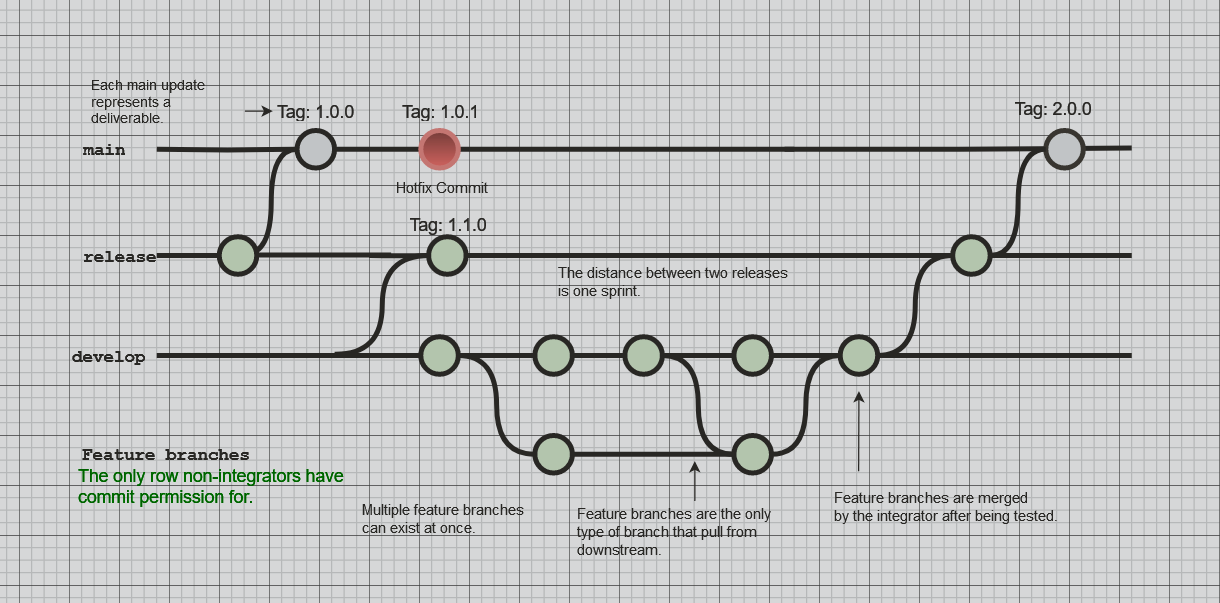
\includegraphics[width=0.9\linewidth]{Figures/git-workflow.png}
    \caption{Git Workflow Representation}
    \label{fig:git-workflow}
    %\vspace{-5mm}
\end{figure*}


% \newpage
\divider

\section{Issues Handling} \label{section: issues handling}

\subsection{Issues Creation}

Issues will be created for each individual feature that needs to be implemented, or necessary fix. These issues will be tracked via Github. A feature branch will be created for each issue, which will share its number for linking purposes. Many issues will be created based on each deliverable at the start of work, but new issues will be added during sprints if a need arises.

\subsection{Issues Tracking}

Github projects will be used to track progress on different issues and pull requests. This will make it easy for the integrator to track pull requests, and for the project manager to understand the current progress at a glance. Issues can be placed one of the below categories, and must move through each category before being considered resolved. If unexpected problems arise (such as a feature failing its testing) it can be moved back to an earlier stage. The categories are as follows:

\textbf{Todo}: Work has not begun on this issue. A feature branch has not yet been created.

\textbf{In Progress}: This issue is being targeted during this sprint. A feature branch has been created and the issue is being actively worked on.

\textbf{Implemented}: The issue-associated feature has been fully implemented and requires testing.

\textbf{Testing}: The feature is actively being tested. This testing is unit testing specific to the feature, overall testing for a release is handled separately.

\textbf{Tested}: The feature has passed all testing. It is awaiting approval and merge by the integrator.

\textbf{Merging}: The integrator is currently working on merging this feature to Develop. Any merge conflicts are resolved during this time, and the code and testing procedures are double-checked by the integrator.

\textbf{Merged}: The integrator has successfully merged the fully tested feature to the Develop branch. It now awaits acknowledgement by the project manager.

\textbf{Done}: The project manager has acknowledged the merged feature and declared it done.

\subsection{Issues Assignment}

Assignment will be handled by the team lead. Issues in the to-do list will be handed to specific developers who will work on them for the duration of a sprint. In general, assignment will occur at the beginning of each sprint. Features will be broken into small pieces, such that each feature is assigned to one developer at a time. Developers can, of course, ask for help, but in general tasks should be well-matched to their abilities, knowledge base, and availability.

\subsection{Pull Request Review Process}

The integrator will manually review all feature pull requests before merging them to Develop. In addition to a basic inspection of the code added, ensuring that it matches the specifications on the linked issue, the integrator will examine the testing performed. If the testing is not adequate, the integrator will request further testing. If the testing is sufficient, the integrator will attempt to merge the feature to Develop.

\subsection{Feature Testing Process}

The feature testing process will depend heavily on which feature is being added. However, testing at the feature level should focus on small-scale unit tests around the code being changed, rather than testing of the overall program. The reason for this approach is that it may be impractical to impossible to test every feature on a large scale. Early on, not enough of the program will be completed for large-scale testing, and later bugs present in other sections of the program may lead to inaccurate test results. Therefore, major features should go through a set of unit tests before their implementation. If the feature will have a large impact on the program overall, then any complete sections should be tested alongside the feature, to ensure that all modules are inter-operating correctly.


% \newpage
\divider

\section{Continuous Integration / Continuous Development (CI/CD)} \label{section: CI-CD}

Because features are being implemented asynchronously, it is important to ensure that all modules work together effectively. However, performing an exhaustive set of tests after every feature implementation is impractical. To maintain quality and safety, CI/CD will be implemented when merging from Develop to Release. Every release will go through a thorough battery of automated tests to ensure it is fully functional and bug-free. If these tests are failed, then the Develop branch will be adjusted and the release will be attempted again.

% \newpage
\divider

% Creates references using the Biblatex 
\bibliographystyle{plain}
\bibliography{General/References.bib}
\newpage

\appendix % Any section after this command will have a letter as an index

% Adds an appendix entry
% \section{Appendix A title} \label{section: appendix A title}
\lipsum[1-8]
% \newpage

\end{document}
